%!TEX root = main.tex
\documentclass[conference, tikz]{IEEEtran}
\IEEEoverridecommandlockouts
% The preceding line is only needed to identify funding in the first footnote. If that is unneeded, please comment it out.

\usepackage{physics}
\usepackage{tikz}
\usepackage{tikz-3dplot}
\usepackage[outline]{contour} % glow around text
\usepackage{xcolor}
\usepackage{multimedia}
% Tikz styles
\colorlet{veccol}{green!50!black}
\colorlet{projcol}{blue!70!black}
\colorlet{myblue}{blue!80!black}
\colorlet{myred}{red!90!black}
\colorlet{mydarkblue}{blue!50!black}
\tikzset{>=latex} % for LaTeX arrow head
\tikzstyle{proj}=[projcol!80,line width=0.08] %very thin
\tikzstyle{area}=[draw=veccol,fill=veccol!80,fill opacity=0.6]
\tikzstyle{vector}=[-stealth,myblue,thick,line cap=round]
\tikzstyle{unit vector}=[->,veccol,thick,line cap=round]
\tikzstyle{dark unit vector}=[unit vector,veccol!70!black]
\usetikzlibrary{angles,quotes} % for pic (angle labels)
\contourlength{1.3pt}

\usepackage{caption}
\usepackage[labelsep=quad,indention=10pt]{subfig}
\usepackage{amsmath,amssymb,amsfonts}
\usepackage{algorithmic}
\usepackage{graphicx}
\usepackage{textcomp}
\usepackage{xcolor}
\usepackage{media9}
\usepackage{float}
\def\BibTeX{{\rm B\kern-.05em{\sc i\kern-.025em b}\kern-.08em
    T\kern-.1667em\lower.7ex\hbox{E}\kern-.125emX}}

\begin{document}

\title{Designing an MPC Controller for a Simplified Rocket Landing Problem}
\author{\IEEEauthorblockN{ Sebastiano Zuddas}
\IEEEauthorblockA{\textit{dept. Automatic Control \& Systems Engineering} \\
\textit{University of Sheffield}\\
Sheffield, United Kingdom \\
sebastianozuddas1@gmail.com}

}

\maketitle

\begin{abstract}
The report discusses the implementation of model-predictive control (MPC) on a simplified rocket landing problem. The MPC is incrementally improved through the report, giving details on design decisions, particularly penalty matrices, constraints, and disturbance rejection. Finally, the report discusses the results obtained, proposing improvements through improving model accuracy and the implementation of tracking an ideal landing trajectory. 
\end{abstract}

\begin{IEEEkeywords}
MPC, Rocket Landing, Model Predictive Control, Control Theory, Control Engineering
\end{IEEEkeywords}

\section{Introduction}
The objective of the assignment is to implement a model-predictive control (MPC) scheme to land a simplified model of a rocket. 
The problem is fundamentally one of 'controllability', ie $x(0) = x_s \rightarrow x(t_f) = 0$. The assignment gives an abstract model, and the model is rewritten for clarity as follows:
\begin{center}
\begin{equation}
    \begin{bmatrix}
        r_x(k+1)\\
        r_y(k+1)\\
        r_z(k+1)\\
        v_x(k+1)\\
        v_y(k+1)\\
        v_z(k+1)\\
    \end{bmatrix}
    =
    \begin{bmatrix}
       1 & 0 & 0 & T_s & 0 & 0\\
       0 & 1 & 0 & 0 & T_s & 0\\
       0 & 0 & 1 & 0 & 0 & T_s\\
       0 & 0 & 0 & 1 & 0 & 0\\
       0 & 0 & 0 & 0 & 1 & 0\\
       0 & 0 & 0 & 0 & 0 & 1
    \end{bmatrix}
    \begin{bmatrix}
        r_x(k)\\
        r_y(k)\\
        r_z(k)\\
        v_x(k)\\
        v_y(k)\\
        v_z(k)\\
    \end{bmatrix}
    +
    \hspace*{2cm}

    \begin{bmatrix}
        \frac{T_s^2}{2m} & 0 & 0\\
        0 & \frac{T_s^2}{2m} & 0\\
        0 & 0 & \frac{T_s^2}{2m}\\
        T_s & 0 & 0\\
        0 & T_s & 0\\
        0 & 0 & T_s
    \end{bmatrix}
    \begin{bmatrix}
        f_x(k)+w_x\\
        f_y(k)+w_y\\
        f_z(k)-mg\\
    \end{bmatrix}
    \label{eq:1}
\end{equation}
\end{center}

The objective is to find the optimal control input $f_x(k), f_y(k), f_z(k)$ such that the state $x(k)$ converges to $\vec x(t_f)=\vec{0}$ in finite time $t_f$. Although it is assumed the system is reachable, it is important to check for controllability. 
Through MATLAB: \verb|Rank = rank(ctrb(A, B))| the system is seen to be controllable and can proceed with designing a controller. 

\section{Design}

\subsection{Controller Design}
Three separate controllers are considered in this report. 
The first controller is an unconstrained, two-stage MPC. The second controller builds on the first and introduces state and input constraints. The third controller further builds on the first two, introducing disturbance rejection (DR).
Firstly, the unconstrained controller design is presented.

\subsubsection{Unconstrained}
The $Q$ and $R$ matrices are chosen as follows:

\[
    Q = \begin{bmatrix}
        5&0&0&0&0&0 \\
        0&5&0&0&0&0 \\
        0&0&100&0&0&0 \\
        0&0&0&1&0&0 \\
        0&0&0&0&1&0 \\
        0&0&0&0&0&100 \\
    \end{bmatrix}
    ;\\ R = I \cdot 0.1 \text{ for }  I \in \mathbb{R}^{3\times 3}
\]

The $Q$ matrix was chosen to prioritise the vertical position and velocity.This represents the high level of importance given to landing at the correct altitude. Similarly, the prioritisation of velocity represents the importance of landing at a velocity that prevents a hard landing.

The lateral positions, ie $r_x$ and $r_y$, are given a lower priority than the vertical position, but a higher priority than the lateral velocity, $v_x$ and $v_y$. It is more important that the landing location is correct before the lateral velocities are accounted for.  

The $R$ matrix was chosen to penalise the control inputs, $f_x$, $f_y$, and $f_z$, equally.
The small value given to $R$, 0.1, represents the low cost associated with expending fuel to control the rocket and encourages the rocket to use fuel to exercise control in all three directions equally. Essentially, control is cheap. 

The horizon length $N$ was chosen to be 5 as it provided a spectral radius of 0.5975, which is well within the stability region of the system.

The poles of the closed-loop system were placed through \verb|K_2 = -place(A, B, [0.01 0.01 0 0.01 0 0])|. The most important poles, ie the poles representing $r_z$, $v_z$ were placed at zero. 
The limitations of the \verb|place()| function meant that not every pole could be set to zero, hence the other poles were set to $0.01$. 

The weighting matrix $P$ was calculated using \verb|P = dlyap((A+B*K_2), Q+K_2'*R*K_2)|. The prediction matrices $F$ and $G$ were generated using the \verb|predict_mats()| function, and the corresponding cost matrices $H$, $L$ and $M$ were generated using the \verb|cost_mats()| function. 
It is assumed at this point that $Q\succeq 0$ and $R \succ 0$ which implies $\vec u^*_N(k) = -H^{-1}\cdot Lx(k)$.

As such, the unique and optimal solution to the optimal control problem is obtained and is through quadratic programming at each time step \verb|Uopt = quadprog(H, L*x)|. 

\subsubsection{Constrained}
The constrained controller builds on the unconstrained controller by introducing state and input constraints. 

The input constraints are chosen as follows:
The linear inequality constraints are based on the brief, and are set as follows:
\begin{center}
\[
    P_x = 
    \begin{bmatrix}
        I_x\\
        -I_x
    \end{bmatrix}
    P_x = 
    \begin{bmatrix}
        I_u\\
        -I_u    
    \end{bmatrix}
    \text{ for } I_x \in \mathbb{R}^{6\times 6} \text{ and }I_u\in \mathbb{R}^{3\times 3}
    \\
    q_x = 
    \begin{bmatrix}
        \frac{r_z}{\tan{\phi}}+50\\
        \frac{r_z}{\tan{\phi}}+50\\
        500\\
        20\\
        20\\
        15\\
        \frac{r_z}{\tan{\phi}}+50\\
        \frac{r_z}{\tan{\phi}}+50\\
        0\\
        20\\
        20\\
        15
    \end{bmatrix}
    q_u =
    \begin{bmatrix}
        f_z\cdot\tan{\theta}\\
        f_z\cdot\tan{\theta}\\
        12\\
        f_z\cdot\tan{\theta}\\
        f_z\cdot\tan{\theta}\\
        0
    \end{bmatrix}
\]
\end{center}

The $r_x \ r_y$ constraints were given in the brief as $|r_x|, |r_y| \le \frac{r_z}{\tan{\phi}}$ where $\phi$ represents the glide slope angle and is chosen as a constant $\phi = 30^\circ = 0.52\text{ rad}$.

The input constraints given in the brief as $|f_x|, |f_y| \le f_z \tan{\theta}$ where $\theta$ represents the maximum allowable angle of the rocket engines, and is chosen as $\theta = 10 ^\circ = 0.17\text{ rad}$.

\begin{figure}[H]
\centering
\tdplotsetmaincoords{60}{110}
\begin{tikzpicture}[scale=1,tdplot_main_coords]
  % AXES
  \coordinate (O) at (0,0,0);
  \draw[thick,->] (0,0,0) -- (1,0,0) node[below left=-3]{$r_x$};
  \draw[thick,->] (0,0,0) -- (0,1,0) node[right=-1]{$r_y$};
  \draw[thick,->] (0,0,0) -- (0,0,1) node[above=-1]{$r_z$};

  % VECTORS
  \draw[vector,red] (0, 0, 0)  -- (0, 0, 0.5) node[right] {$f_z$};
\end{tikzpicture}
\caption{$f_z$ on the $z$ axis.} \label{tikz:axes}
\end{figure}

Figure \ref{tikz:axes} provides a visualization of how $f_z$ acts on the point mass. Overall, this permits the implementation of Algorithm 6.1, pg. 102 from \cite{test}, since all the relevant optimal control and constraint matrices have been defined. The constraint matrices are obtained in code through \verb|constraint_mats()|. 

Disturbances are included in the simulation despite no DR implementation, mainly to be able to contrast the results and demonstrate the implementation of DR.

\subsubsection{Disturbance Rejection}
Rank, reachability, and observability tests were performed on $B, E$ and the two pairs $(A, B); (C, A)$ and it was found that DR was possible. 

The DR controller builds on both the unconstrained and constrained controllers. No reference tracking is included in the following controller. 

Only wind disturbance is considered, and is modelled as a sinusoidal signal as follows:
\[
    \vec{w}(k)
    =
    \begin{bmatrix}
        \sin{\frac{50}{k}}\\
        \cos{\frac{50}{k}}\\
        0
    \end{bmatrix}
\]
The use of a sinusoidal disturbance is intended to represent the changing wind speeds as the rocket descends through the atmosphere. The sinusoidal functions were chosen to be out of phase to yield visibly different results. 
\\
In terms of controller design, equation \ref{eq:1} is rewritten as follows:
\[
    \begin{cases}
    x(k+1) = Ax(k) + Bu(k) + Ew(k)\\
    y(k) = Cx(k) + Fd(k)
    \end{cases}
\]
where $E = B$ and $F=0$ since output disturbances are negated, hence:
\[
    \begin{cases}
        x(k+1) = Ax(k) + B(u(k) + w(k))\\
        y(k) = Cx(k)
    \end{cases}
\]

It is now possible to formulate the $T$ matrix to find $x_{ss};u_{ss}$.
\[
    T = 
    \begin{bmatrix}
        I-A & -B\\
        C & 0
    \end{bmatrix}
\]
In this case, $C \in \mathbb{R}^{6 \times 6} \land B \in \mathbb{R}^{6 \times 3} \therefore p < m \iff 3 < 6$.
Similarly, it is seen that $T$ is full row rank, confirming that for any pair $ (r, d) \ \exists$ a pair $(x_{ss}, u_{ss})$.
As such, $x_{ss};u_{ss}$ are given by:
\[
    \begin{bmatrix}
        x_{ss}(k)\\
        u_{ss}(k)
    \end{bmatrix}
    =
    T^{-1}
    \begin{bmatrix}
        B\cdot \vec w(k)\\

        0
    \end{bmatrix}
\]
From this result, the deviation variables become $ z := x - x_{ss}; v := u - x_{ss}$. 
As a result, $v^*(k|k)$ is calculated through \verb|quadprog(H, L*z, qc+Sc*z)| at each iteration.

\subsection{Experiment Setup}
The mass of the rocket is simplified and assumed to be constant for all experiments, and is chosen as $m = 1\text{ kg}$.

The starting parameters for each experiment are as follows:
\[
    \vec x(0)
        =
        \begin{bmatrix}
            600\\
            600\\
            500\\
            5\\
            5\\
            -15\\
        \end{bmatrix}
        \land
        \vec u(0)
        = \vec 0
\]
These starting conditions are the limits of what the assignment permits, i.e a maximum starting altitude of 500m, and  maximum lateral distances of 600m.

\pagebreak
\section{Results}
\subsection{Constrained}
\begin{figure}[H]
    \centering
    \begin{subfigure}{\columnwidth}
        \centering
        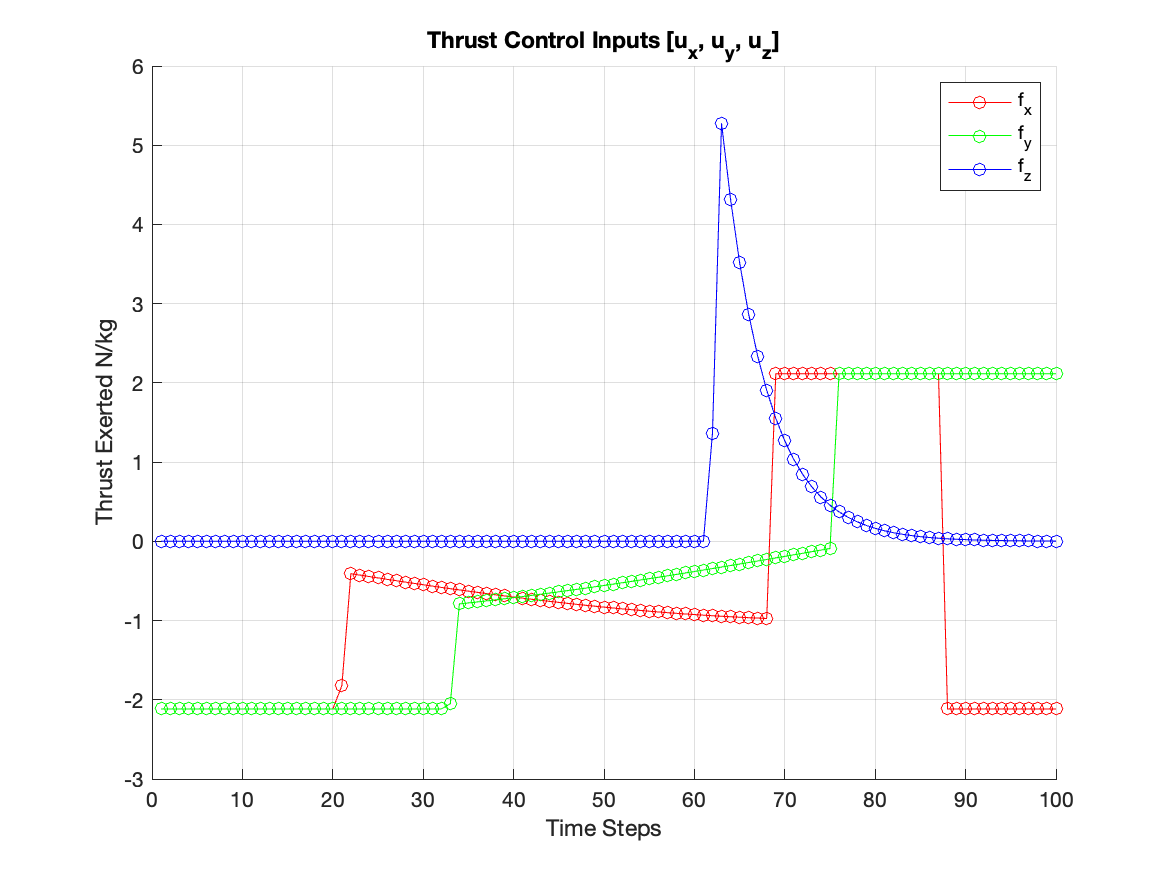
\includegraphics[width=\columnwidth]{Figures/new/Constrained_input_plot.png}
        \caption{Constrained Thrust Control Input}
        \label{const:control_in}
    \end{subfigure}
    \begin{subfigure}{\columnwidth}
        \centering
        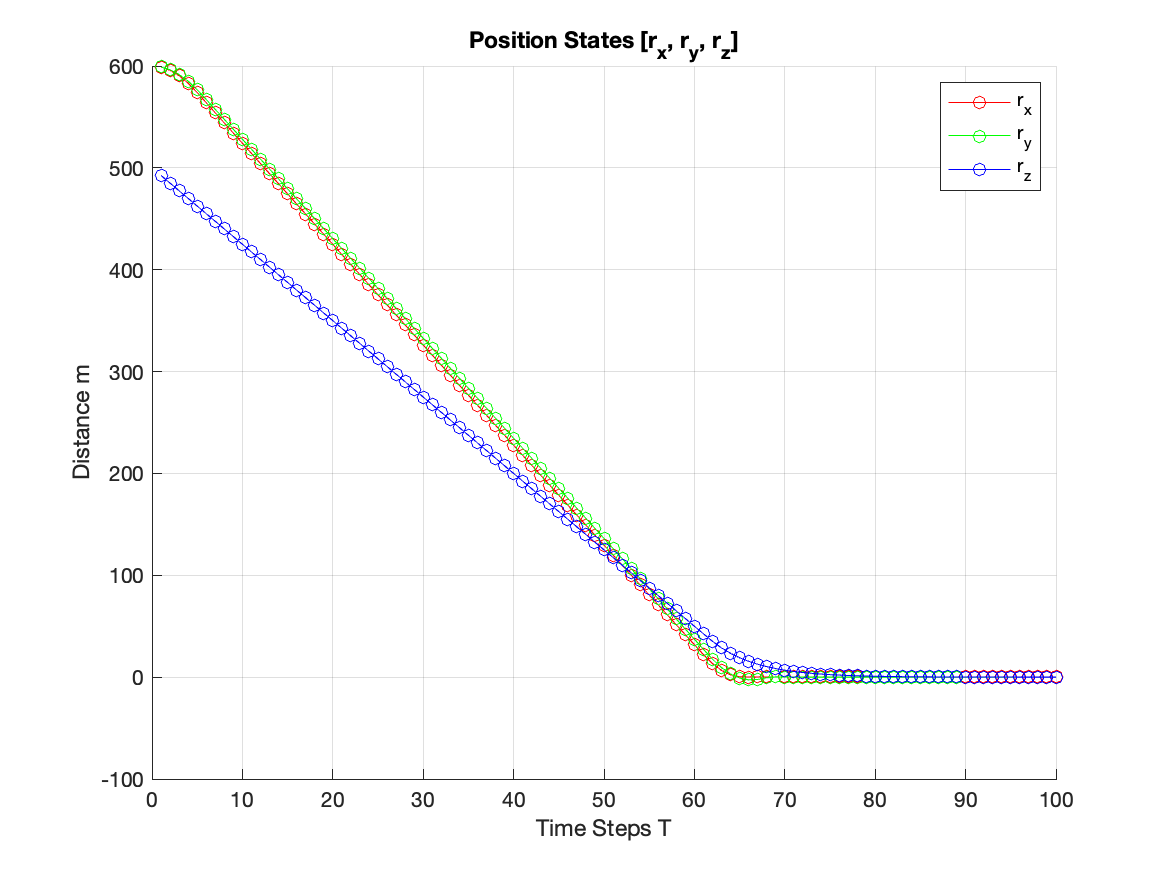
\includegraphics[width=\columnwidth]{Figures/new/Constrained_position_state_plot.png}
        \caption{Constrained Position State Plot}
        \label{const:pos_state}
    \end{subfigure}
    \begin{subfigure}{\columnwidth}
        \centering
        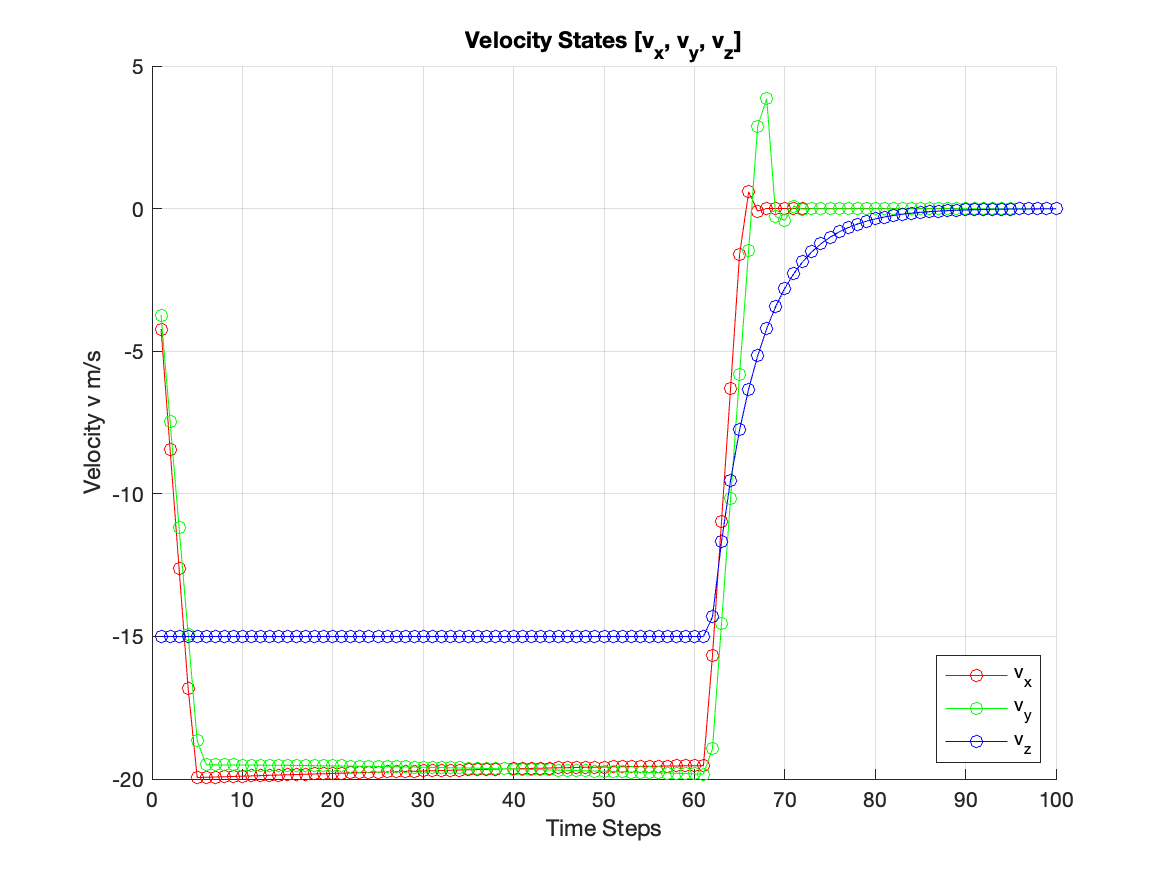
\includegraphics[width=\columnwidth]{Figures/new/Constrained_velocity_state_plot.png}
        \caption{Constrained Velocity State Plot}
        \label{const:vel_ss}
    \end{subfigure}
\end{figure}
\subsection{Disturbance Rejection}
\begin{figure}[H]
    \centering
    \begin{subfigure}{\columnwidth}
        \centering
        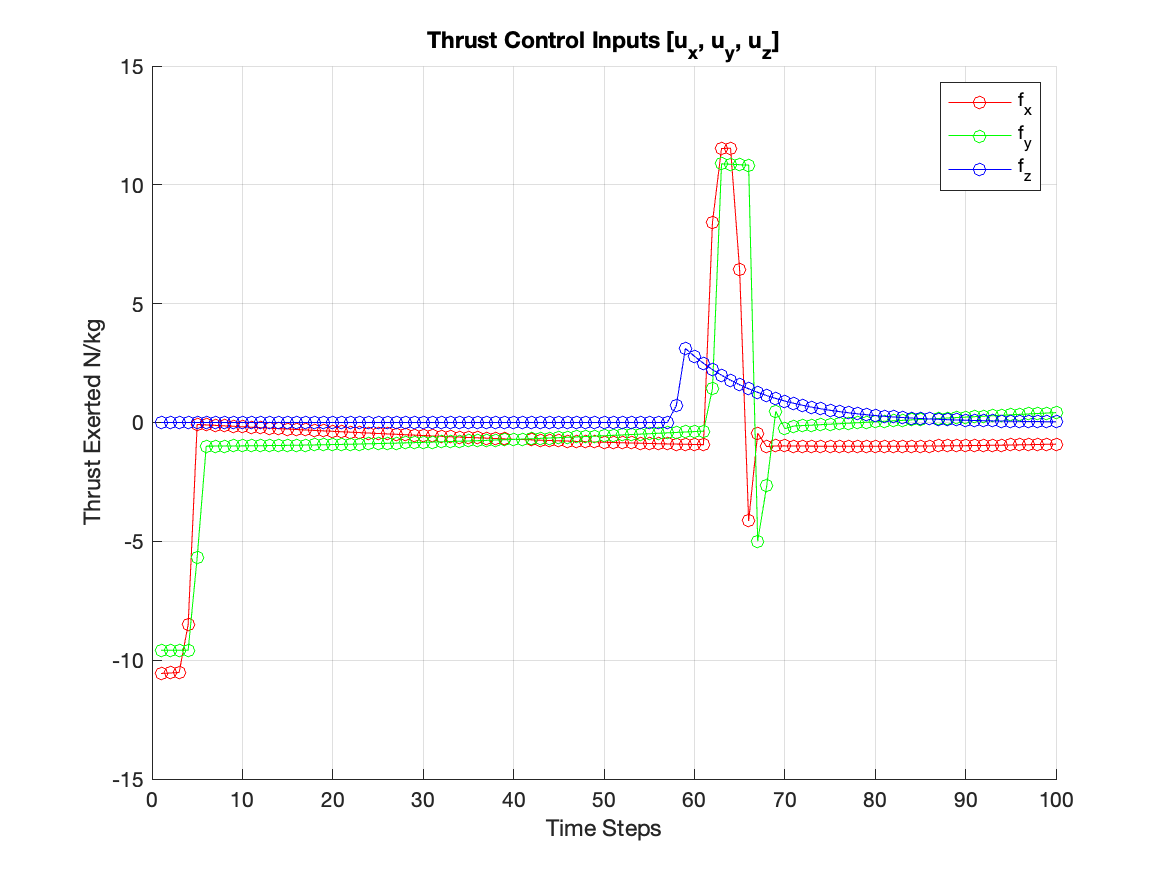
\includegraphics[width=\columnwidth]{new_final_figs/DR_Constrained_input_plot.png}
        \caption{Disturbance Rejection Thrust Control Input}
        \label{DR:control_in}
    \end{subfigure}
    \begin{subfigure}{\columnwidth}
        \centering
        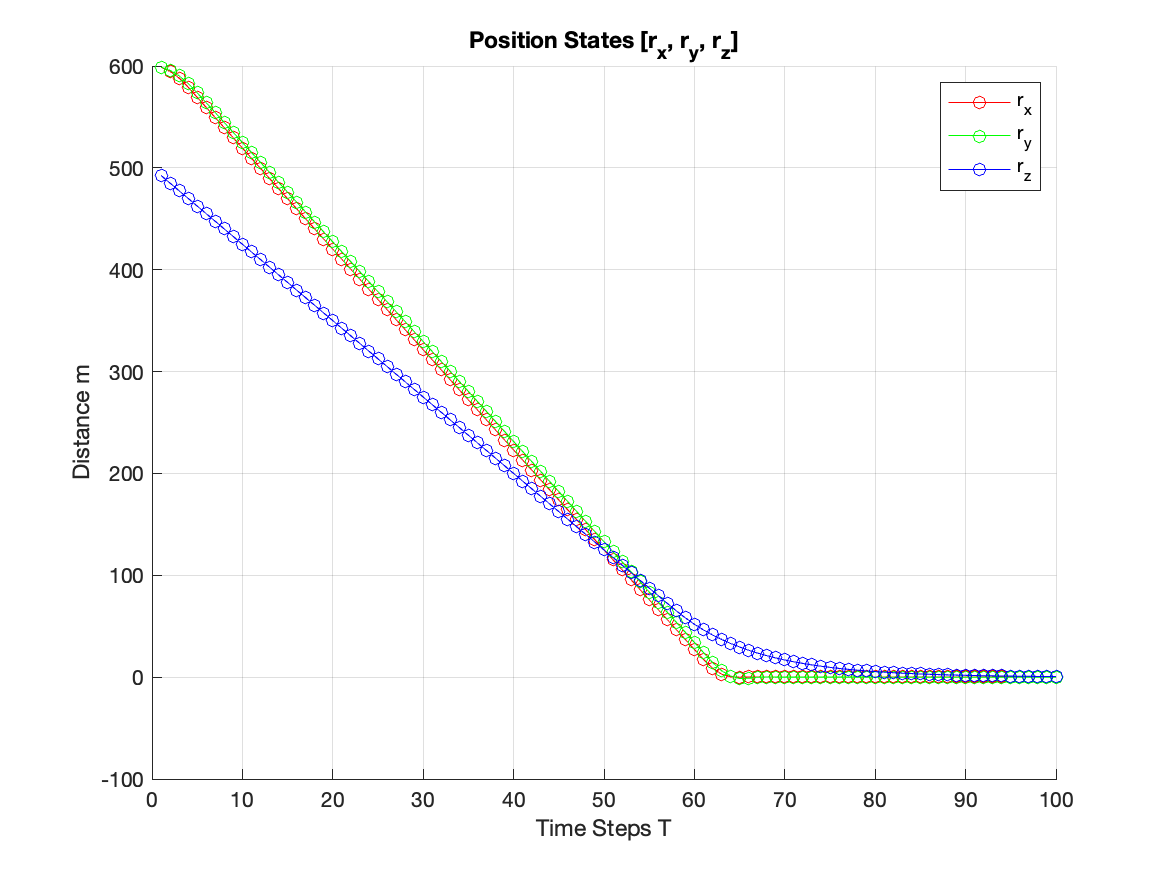
\includegraphics[width=\columnwidth]{new_final_figs/DR_Constrained_position_state_plot.png}
        \caption{Disturbance Rejection Position State Plot}
        \label{DR:pos_state}
    \end{subfigure}
    \begin{subfigure}{\columnwidth}
        \centering
        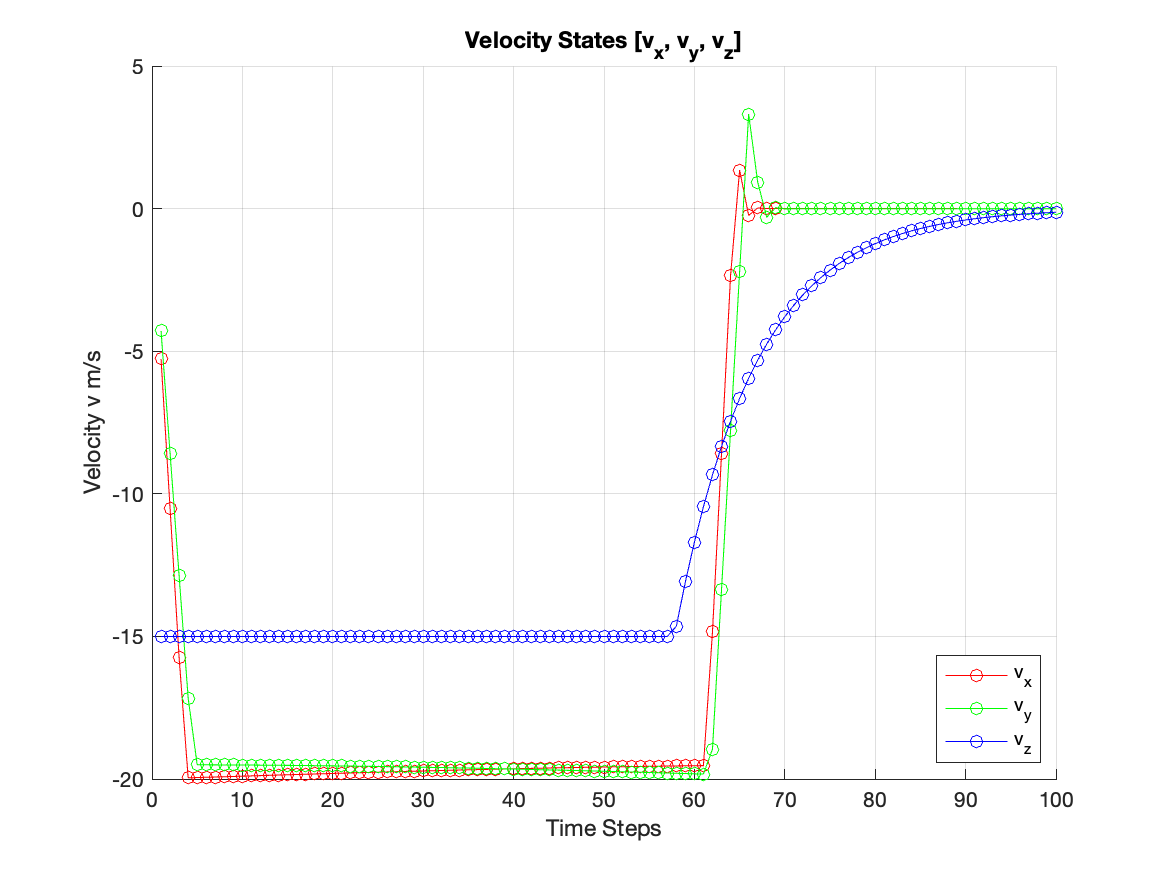
\includegraphics[width=\columnwidth]{new_final_figs/DR_Constrained_velocity_state_plot.png}
        \caption{Disturbance Rejection Velocity State Plot}
        \label{DR:vel_ss}
    \end{subfigure}
\end{figure}

\section{Analysis \& Discussion}
Due to the limitations to the number of pages, the analysis will mainly discuss the effectiveness of the controllers using constraints and DR. Results from the unconstrained controller can be found in the appendix.

\subsection{Similarities}
Considering figures \ref{unconst:pos_state} and \ref{DR:pos_state}, it is clear that both controllers are capable of landing the point mass at $\vec x(t_f) = [0 \ 0 \ 0]^T$. Similarly, both controllers land the rocket smoothly; looking at figures \ref{const:control_in} and \ref{DR:control_in} the $u_z$ value shows a spike in thrust control outputted starting at $k=60$ for the constrained controller and $k\approx58$ for the DR controller.

Both controllers prioritise the coordination of the $r_x, r_y$ position states before the eventual landing of the point mass by decreasing the $r_z$ state to zero. This essentially corresponds to the rocket aligning above the launch pad before the rocket eventually descends. Both controllers achieve lateral stability at the same value of $k=70$. 

Both controllers also have the same landing burn pattern, hence they exhibit the same curves through the z-axis for both velocity and position. 
Both controllers can be seen to have thrust controls that attempt to counter the sinusoidal disturbances throughout the simulation, demonstrated by figures \ref{const:control_in} and \ref{DR:control_in}. Disturbances can also be seen in the other figures but they are less obvious, especially in figures \ref{const:pos_state} and \ref{DR:pos_state}. 

\subsection{Differences}
The most obvious difference between the two controllers is seen when approaching the landing burn.
The constraint controller demonstrated a more abrupt control scheme when adjusting thrust inputs before landing, at approximately $k = 60$ on figure \ref{const:control_in}. At $k\approx70$, a more abrupt dip is also observed in the constraint controller when compared to figure \ref{DR:control_in}. Similarly, the abruptness in the control translates to more abrupt changes in velocities when looking at figures \ref{const:vel_ss} and \ref{DR:vel_ss}. 

The DR controller starts the landing burn earlier and ends the landing burn later than the constraint controller.

Finally, it is clear that the DR controller successfully rejects disturbances more effectively than the constraint controller, when observing the landing phase in figure \ref{DR:pos_state}, paying particular attention to $r_z$ at $k\approx 90 \rightarrow 100$

\subsection{Discussion}
The selection of the $Q$ matrix elements in the way it has prioritised the position states $\vec r(k)$ seems to have been successful in its implementation, as is seen by the adjustment for $r_x$ and $r_y$ before the landing of the point mass. A similar conclusion can be drawn for $\vec v(k)$. 

The cheap control assigned to the $R$ matrix seems to have led to abrupt changes in the input states, leading to large spikes in thrust control outputs, visible in both controllers. Although this setting permits a successful landing, it may not be applicable in a real-world setting, since the change in the applied output force $\vec f(k)$ may be dangerous. A way to mitigate this could be to add more detail to the original model, modifying $A$ and $B$ such that the rates of change of engine thrust are accounted for, and setting their constraints appropriately. Setting a higher value for $R$ may not be effective since the values would result in less control action at more 

Although the constraints matrices account for maximum limits, they do not change through the simulation, nor do they account for the respective angles at each point $\theta(k)$ and $\phi(k)$. Although the point mass was successful at landing, it did not follow the appropriate trajectory, as can be seen in figures \ref{const:3D} and \ref{DR:3D} in the appendix. The simulation would then be rendered more realistic should $\theta(k)$ and $\phi(k)$ be accounted for. Similar to the rate of change of thrust, there would be limitations on engine actuation, and the rate of change of $\theta(k)$ and $\phi(k)$ could be modelled, making simulation more realistic. 

The implementation of disturbance rejection was successful, but only in part. There is little visual difference between the constrained and the DR figures, despite the successful implementation of $z = x - x_{ss}$ and $v = u - x_{ss}$ in code. This may in part be attributed to setting $F = 0$. Nonetheless, both controllers seem to account for disturbances, seen in figures \ref{DR:pos_state} and \ref{DR:control_in}. Further disturbances could also be modelled, such as noise on control signals.

Reference tracking was not implemented, but would have increased the realism of the simulation significantly, by setting a reference trajectory for the point mass to follow. This would have led to a more appropriate landing trajectory, and consequently a safer landing. 

\subsection{Overall Performance \& Recommendations}
Both controllers adequately solve the simplified rocket landing problem. Many iterations of the controllers were attempted, but the demonstrated results displayed are those where the most ideal behaviour was found. 

To increase the realism of the model, rates of change of various parameters could be included, such as the $\delta \theta(k)$, $\delta \phi(k)$, $\nabla \vec f(k)$ and their various constraints. Similarly, a more thorough implementation of DR and reference tracking would add to the credibility of the controller. 

\section{Conclusion}
Overall, the simplified rocket landing problem in the context presented was solved through the implementation of an MPC on the point mass. The most advanced controller presented featured DR, and presented the most appropriate descent and landing profile of the three controllers developed. Some recommendations were made to improve the model through adding reference tracking of an ideal landing, along with increasing model detail by adding rates of change of relevant angles both in the glide slope and the engine angle.  

\bibliographystyle{ieeetr} % Add the bibliography style
\bibliography{references.bib}

\appendix

\subsection{Unconstrained}
\begin{figure}[H]
    \centering
    \begin{subfigure}{\columnwidth}
        \centering
        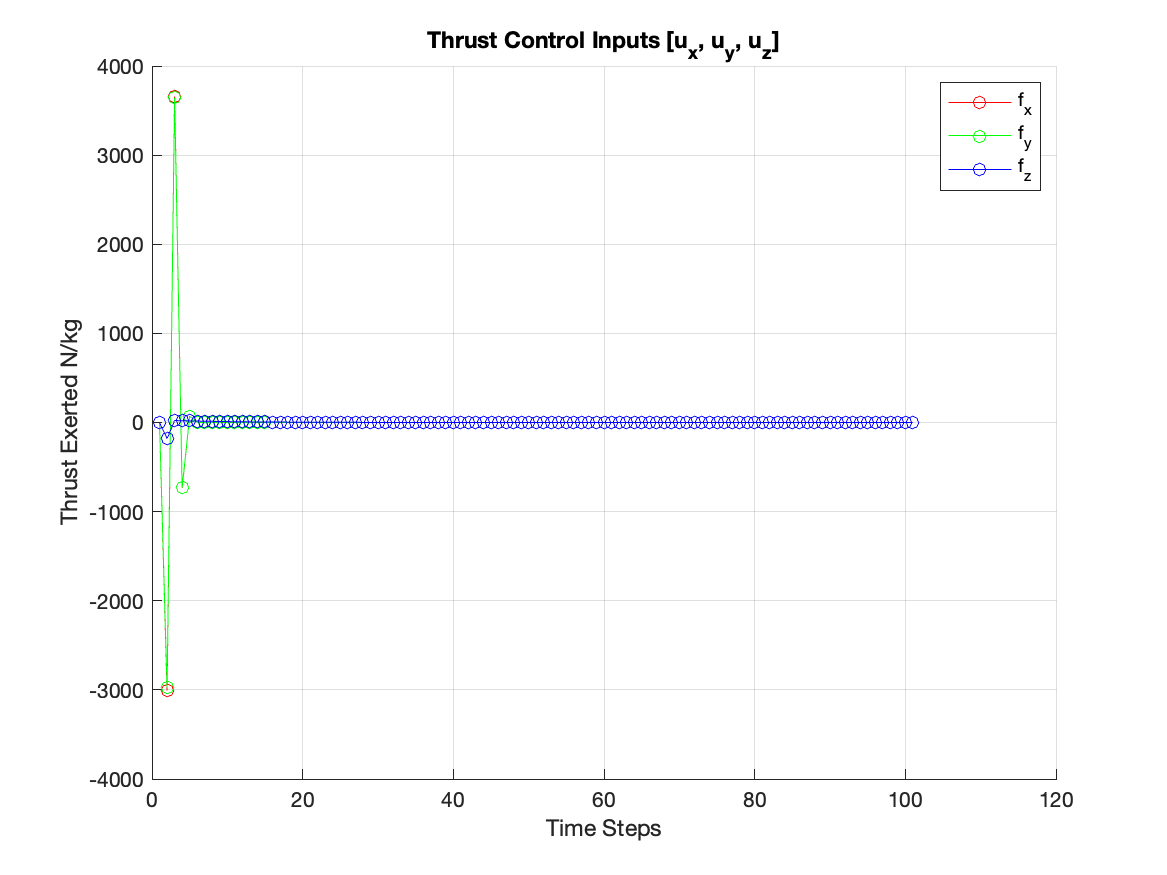
\includegraphics[width=\columnwidth]{new_final_figs/Unconstrained_input_plot.png}
        \caption{Unconstrained Thrust Control Input}
        \label{unconst:control_in}
    \end{subfigure}
    \begin{subfigure}{\columnwidth}
        \centering
        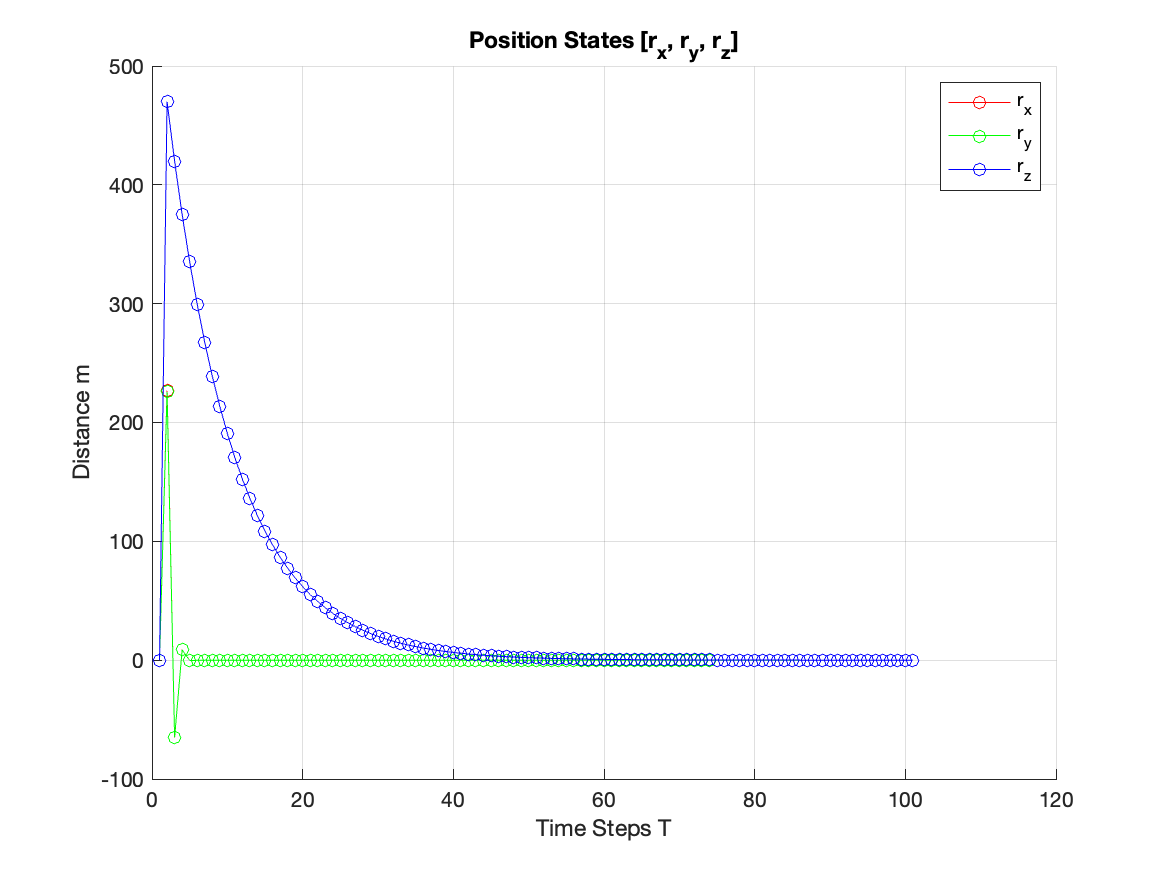
\includegraphics[width=\columnwidth]{new_final_figs/Unconstrained_position_state_plot.png}
        \caption{Unconstrained Position State Plot}
        \label{unconst:pos_state}
    \end{subfigure}
    \begin{subfigure}{\columnwidth}
        \centering
        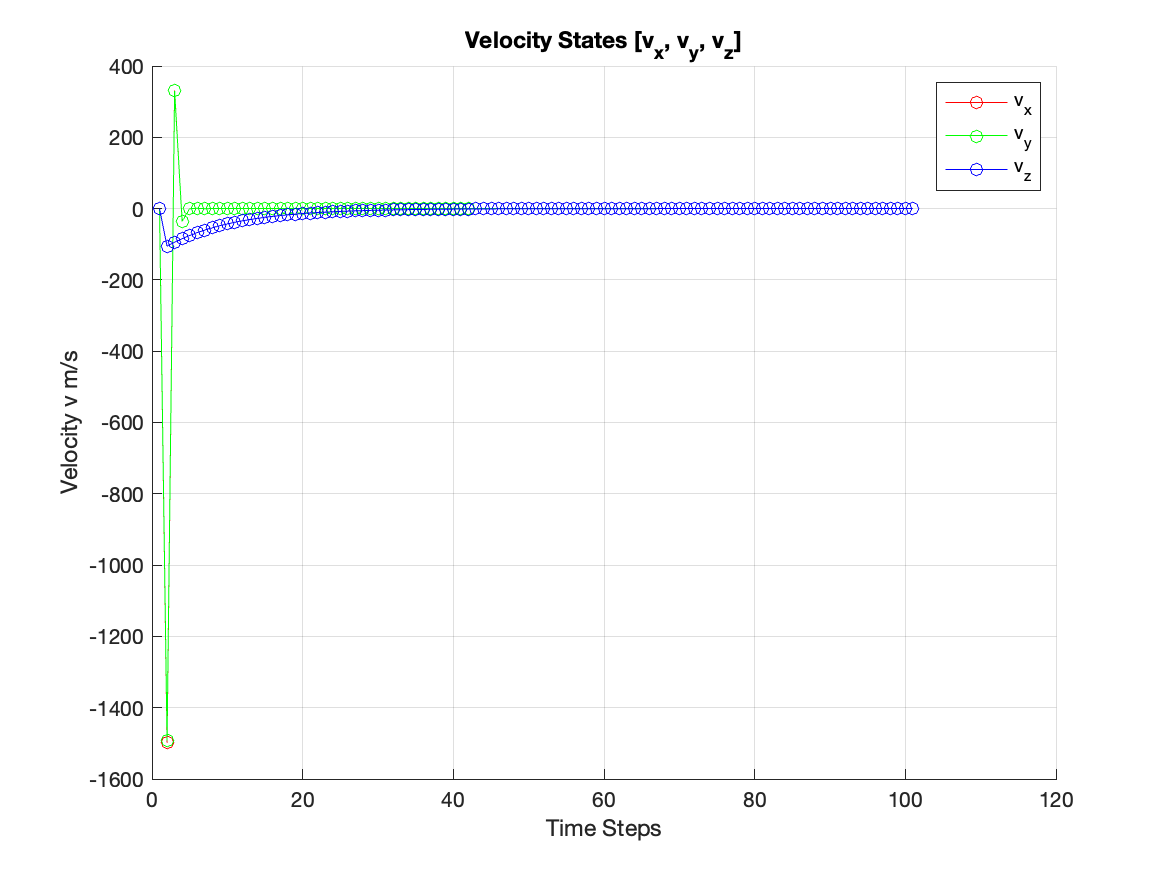
\includegraphics[width=\columnwidth]{new_final_figs/Unconstrained_velocity_state_plot.png}
        \caption{Unconstrained Velocity State Plot}
        \label{unconst:vel_ss}
    \end{subfigure}
\end{figure}

\subsection{3D Landing Plots}

    \begin{figure}[H]{\columnwidth}
        \centering
        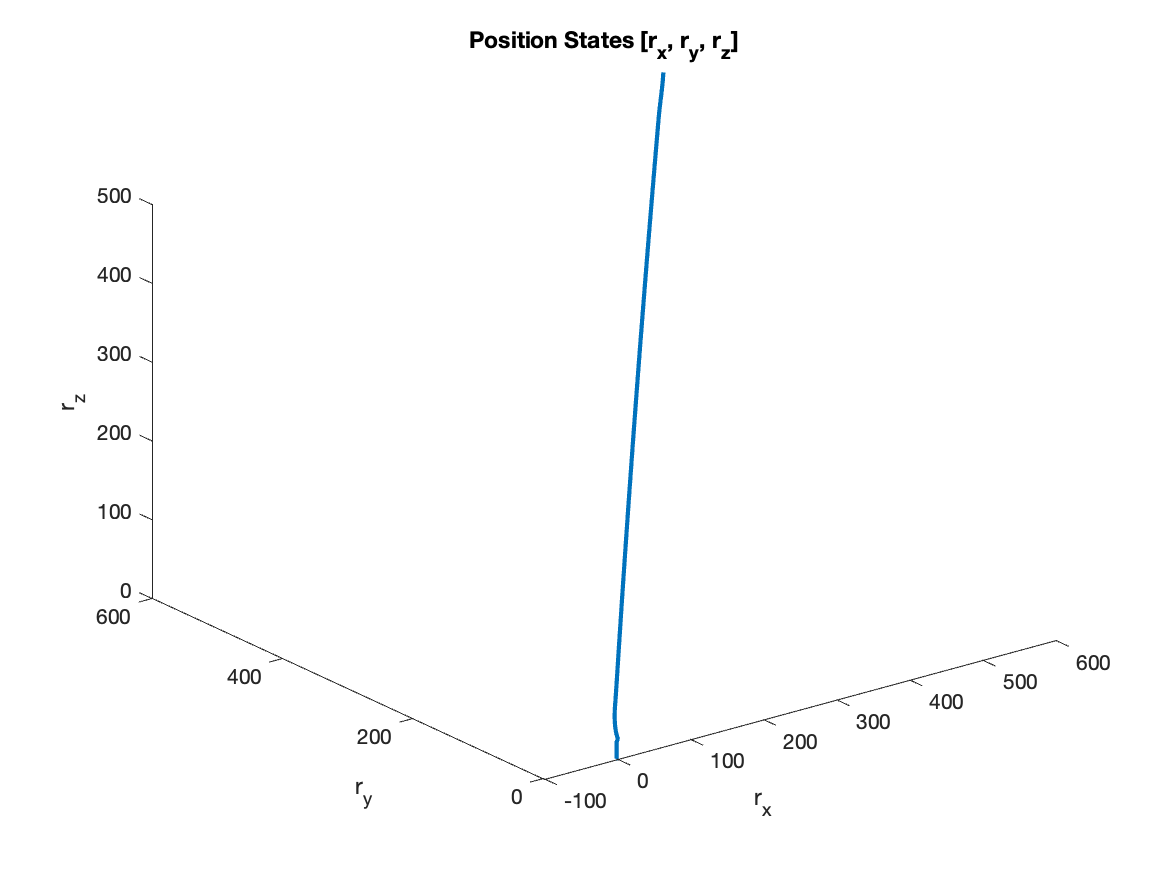
\includegraphics[width=\columnwidth]{new_final_figs/Constrained_position_3D_plot.png}
        \caption{Constrained 3D Landing Plot}
        \label{const:3D}
    \end{figure}
    
    \begin{figure}[H]{\columnwidth}
        \centering
        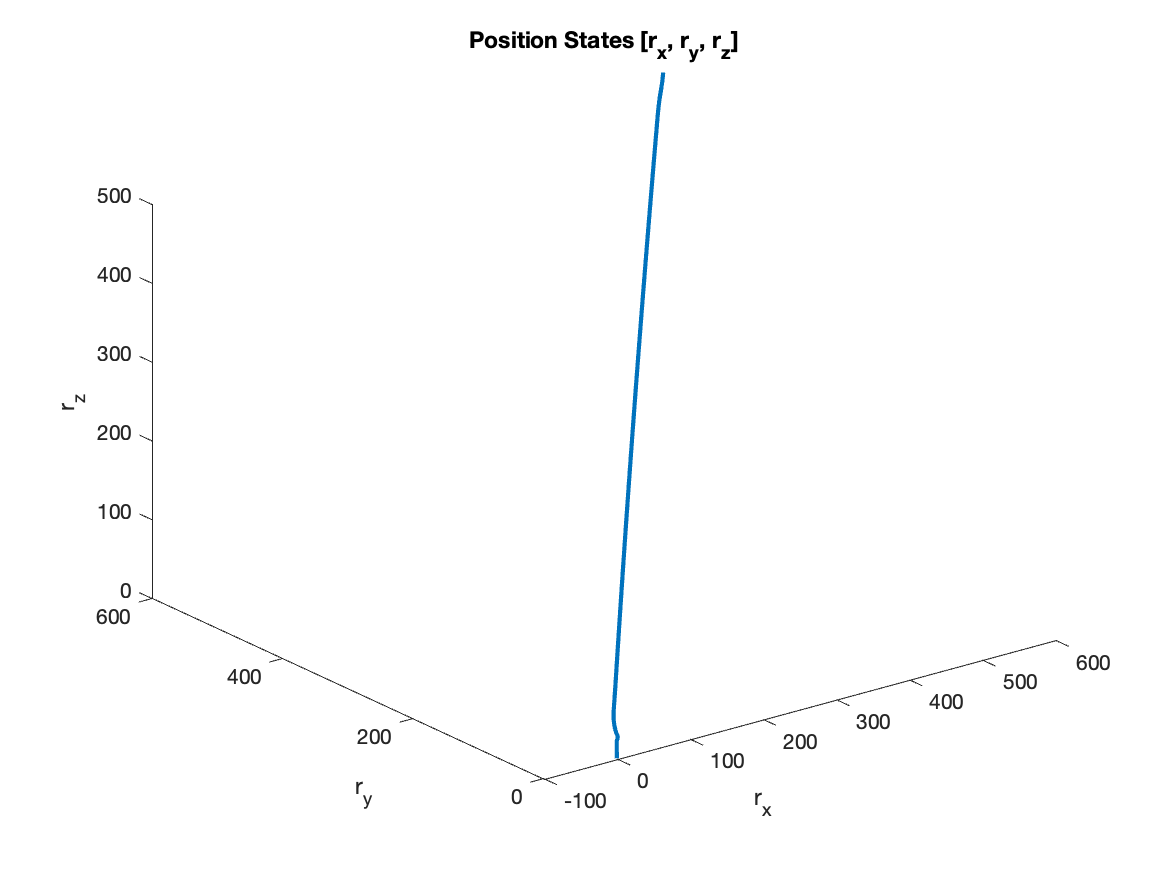
\includegraphics[width=\columnwidth]{new_final_figs/DR_Constrained_position_3D_plot.png}
        \caption{Disturbance Rejection 3D Landing Plot}
        \label{DR:3D}
    \end{figure}




\end{document}
